\subsection{Discussion}\label{subsec:discussion}

\begin{figure}[t!]
\centering
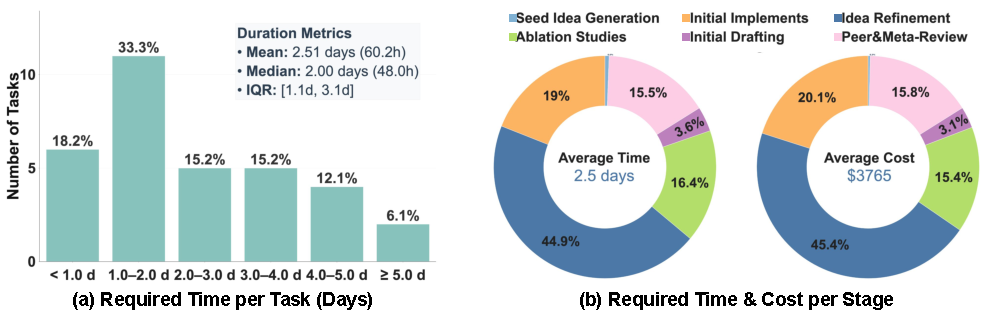
\includegraphics[width=\linewidth]{figures/scientisttwo_cost.pdf}
\caption{\textbf{Computational cost of \sname.} \textbf{(a)} \sname~requires 2.5 days on average to improve a single paper. \textbf{(b)} Idea refinement accounts for the majority of overall time and computational cost, primarily driven by iterative idea evolution and experimental execution.}
\label{fig:cost}
\end{figure}
\noindent\textbf{Cost Analysis.} For cost analysis, we analyze on the 33 target problems sourced from NeurIPS 2025 papers. As shown in Figure~\ref{fig:cost}(a), \sname~requires an average of 2--3 days to complete the entire research cycle, demonstrating significantly faster execution compared to human researchers and substantially accelerating the exploration of new research directions. Figure~\ref{fig:cost}(b) highlights that the majority of execution time is concentrated in the Idea Refinement, Dynamic Peer-Review, and Meta-Review stages. This overhead stems from iterative benchmark evaluation and code execution—traditionally the most time-consuming phase in empirical research. Across the full pipeline, \sname~incurs an average cost of \$3765, including token usage costs and virtual machine costs (Figure~\ref{fig:cost}(b), right). Cost expenditure increases proportionally to execution time, which is primarily due to long-term experimentation and the large amount of context and generation requirements.

\begin{table}[t!]
\centering
\caption{\textbf{Iterative Frontier Expansion.} Sequential discovery results where \sname~uses its own newly discovered state-of-the-art method as context to drive further algorithmic improvements.}\label{tab:seq_scientisttwo}
\begin{tabular}{lll}
\toprule
\textbf{Frontier} & \textbf{Researcher} & \textbf{Method}\\
\midrule
Human Baseline & Human & \citet{jiang2026incremental}\\
\midrule
&&{$\downarrow$ \textit{Relative Gain}: 10.9\%}\\
\rowcolor{Gray}First Iteration & \textbf{\sname~(Ours)} & \textbf{VD-STrans} (\textit{Rating: 6.5})\\
&&{$\downarrow$ \textit{Relative Gain}: 9.6\%}\\
\rowcolor{Gray}Second Iteration & \textbf{\sname~(Ours)} & \textbf{BXT-Transducer} (\textit{Rating: 5.6})\\
&&{$\downarrow$ \textit{Relative Gain}: 8.2\%}\\
\rowcolor{Gray}Third Iteration & \textbf{\sname~(Ours)} & \textbf{SBR-Transducer} (\textit{Rating: \textbf{7.1}})\\
\bottomrule
\end{tabular}
\end{table}
\noindent\textbf{Iterative Frontier Expansion.}
Having demonstrated that \sname~surpasses human-designed baselines, a natural follow-up question is whether \sname~can iteratively compound these gains—namely, can it use its own newly discovered state-of-the-art solutions as priors to discover even better methods? 
As a positive answer, as summarized in Table~\ref{tab:seq_scientisttwo}, \sname~initially discovers VD-STrans, achieving a 10.9\% improvement over the existing state of the art for incremental Byte Pair Encoding (BPE) tokenization \citep{jiang2026incremental}. When VD-STrans is subsequently provided as context in the next discovery cycle, \sname~generates BXT-Transducer, yielding an additional 9.6\% relative improvement over VD-STrans. Moreover, in the third iteration, \sname~proposes SBR-Transducer, again yielding an additional 8.2\% improvement over BXT-Transducer. These results demonstrate that \sname~is capable of compounding discovery, sequentially pushing algorithmic performance beyond both human baselines and its own solutions.

\begin{table}[t]
\centering
\small
\caption{\textbf{Human Reviewers Evaluation.} Standalone scores represent mean absolute ratings for \sname~on a 1--5 Likert scale (> 3.0 indicates positive endorsement). Comparative scores represent relative preference between human-written and \sname-generated papers on a 1--5 scale (3.0 = Parity, > 3.0 favors \sname).}
\label{tab:human_eval}
\begin{tabular}{lcc}
\toprule
\textbf{Focus Aspect} & \textbf{Standalone} & \textbf{Relative to Human} \\
\midrule
Introduction (Motivation \& Related Works) & 4.2 & 3.1 (Human < \sname)\\
Method (Soundness \& Algorithmic Rigor) & 4.1 & 2.9 (Human > \sname)\\
Experiment (Baseline \& Benchmark) & 4.0 & 3.5 (Human < \sname)\\
Experiment (Ablations) & 4.3 & 3.3 (Human < \sname)\\
Experiment (Insight \& Limitation Analysis) & 4.0 & 3.3 (Human < \sname)\\
Overall (Scientific Maturity \& Top-Tier Venue Readiness) & 3.7 & 3.0 (Human = \sname)\\
\bottomrule
\end{tabular}
\end{table}
\noindent\textbf{Human Evaluation.} To evaluate the research quality of manuscripts produced by \sname, we conducted a human expert evaluation across 33 papers generated from NeurIPS-derived problems, evaluated by 9 experienced human reviewers. Reviewers first scored each \sname-generated paper standalone on a 1--5 Likert scale across six research dimensions. As shown in Table~\ref{tab:human_eval}, \sname~consistently received positive endorsements across all evaluated criteria, achieving notable strengths in ablation design. Furthermore, in pairwise comparative assessments against accepted human-authored papers, \sname~achieved overall parity and was favored in experimental execution—specifically in benchmark breadth. While human researchers retained a slight advantage in methodological rigor, the results demonstrate that \sname~is capable of producing publication-grade manuscripts competitive with human-authored papers at top-tier venues.

\begin{figure}[t!]
\centering
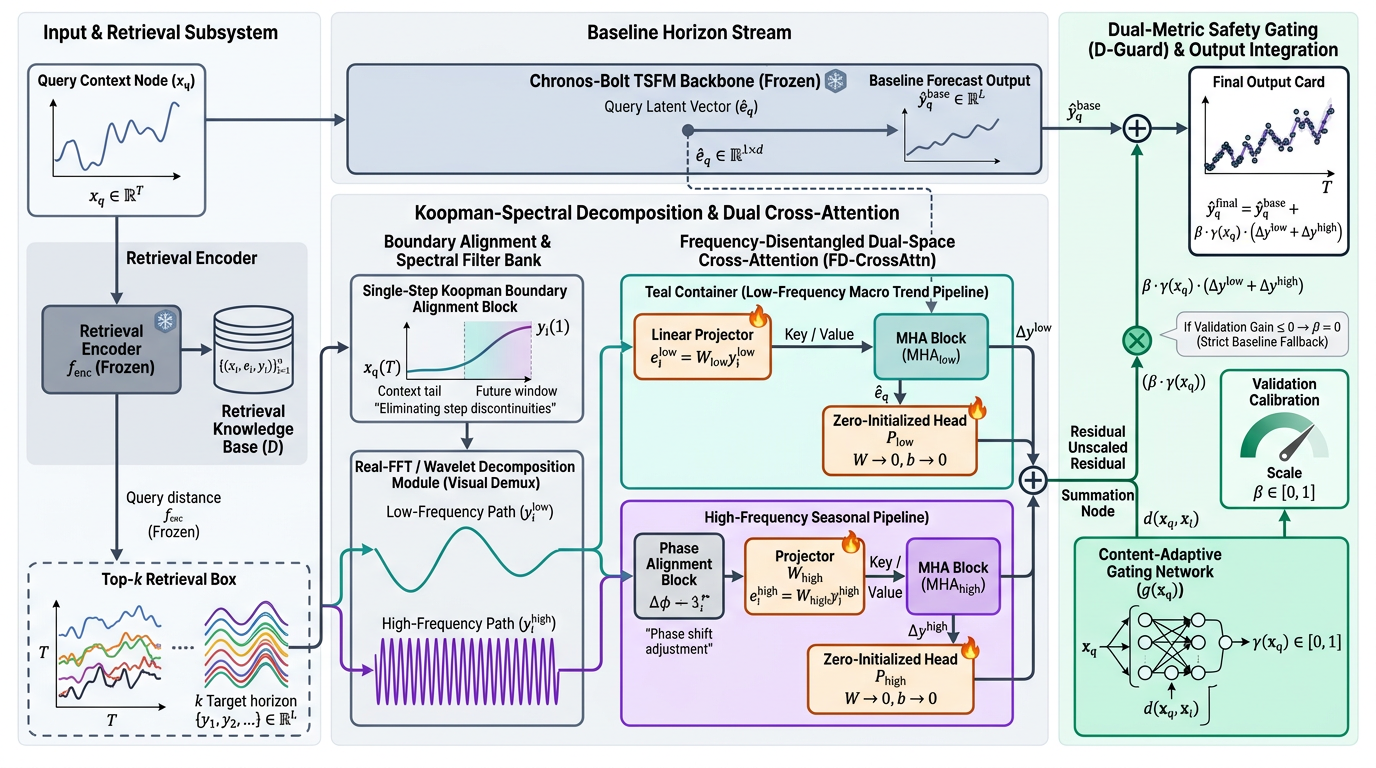
\includegraphics[width=\linewidth]{figures/fig_framework_architecture.jpg}
\caption{\textbf{Case Study: Main Figure of DynaSpec-RAG developed by \sname.} Overall architecture of the DynaSpec-RAG framework for zero-shot time series forecasting.}
\label{fig:ts_rag}
\end{figure}
\begin{table}[t!]
\centering
\caption{\textbf{Case Study: Main Results of DynaSpec-RAG developed by \sname.} Zero-shot long-term forecasting performance ($T=512, L=64$) across seven benchmarks, reported as MSE / MAE (lower is better). Best results are in \textbf{bold}, second-best are \underline{underlined}. ``---'' indicates datasets present in a model's pretraining corpus for which zero-shot numbers are omitted.}
\label{tab:ts_rag}
\resizebox{\textwidth}{!}{%
\begin{tabular}{lcccccccc}
\toprule
\textbf{Method} & \textbf{DynaSpec-RAG} & \textbf{TS-RAG} & \textbf{Chronos-Bolt B} & \textbf{MOMENT} & \textbf{TTM B} & \textbf{Moirai B} & \textbf{TimesFM} & \textbf{Chronos B} \\
\midrule
ETTh1 & \textbf{0.3467} / \underline{0.3627} & \underline{0.3557} / \textbf{0.3624} & 0.3616 / 0.3650 & 0.3920 / 0.4110 & 0.3619 / 0.3710 & 0.3686 / 0.3835 & 0.4254 / 0.3825 & 0.4217 / 0.3806 \\
ETTh2 & \textbf{0.2399} / \textbf{0.2970} & \underline{0.2451} / \underline{0.2982} & 0.2517 / 0.2992 & 0.2742 / 0.3327 & 0.2531 / 0.3032 & 0.2547 / 0.3053 & 0.2894 / 0.3233 & 0.2659 / 0.3136 \\
ETTm1 & \textbf{0.2803} / \textbf{0.3090} & \underline{0.2906} / \underline{0.3114} & 0.3109 / 0.3185 & 0.3506 / 0.3834 & 0.3152 / 0.3248 & 0.5399 / 0.4322 & 0.3321 / 0.3326 & 0.3935 / 0.3695 \\
ETTm2 & \textbf{0.1428} / \textbf{0.2219} & \underline{0.1466} / \underline{0.2231} & 0.1487 / 0.2236 & 0.1703 / 0.2579 & 0.1511 / 0.2405 & 0.1958 / 0.2687 & 0.1703 / 0.2552 & 0.1663 / 0.2522 \\
Weather & \textbf{0.1397} / \textbf{0.1749} & \underline{0.1454} / \underline{0.1771} & 0.1525 / 0.1825 & 0.1801 / 0.2384 & 0.1543 / 0.1893 & 0.1711 / 0.1912 & --- / --- & 0.1897 / 0.2107 \\
Electricity & 0.1135 / 0.2059 & \textbf{0.1120} / \textbf{0.2002} & \underline{0.1132} / \underline{0.2004} & 0.1967 / 0.3028 & 0.1715 / 0.2643 & 0.1832 / 0.2814 & --- / --- & 0.1460 / 0.2237 \\
Exchange & \textbf{0.0615} / \textbf{0.1704} & \underline{0.0627} / \underline{0.1718} & 0.0673 / 0.1780 & 0.0979 / 0.2059 & 0.0657 / 0.1725 & 0.0663 / 0.1720 & 0.0695 / 0.1802 & 0.0831 / 0.1879 \\
\midrule
\textbf{Average} & \textbf{0.1892} / \textbf{0.2488} & \underline{0.1940} / \underline{0.2492} & 0.2008 / 0.2525 & 0.2374 / 0.3046 & 0.2104 / 0.2665 & 0.2542 / 0.2906 & 0.2573 / 0.2948 & 0.2380 / 0.2769 \\
\bottomrule
\end{tabular}}
\end{table}
\noindent\textbf{Case Study.} Prior retrieval augmented forecasting methods \citep{ning2025tsrag} attempt to improve future predictions by fetching similar historical trajectories from external databases, but they treat these retrieved curves as single, indivisible blocks. Such approach creates three critical bottlenecks: it introduces unnatural jumps right at the boundary where current observations end and the forecast begins, it tangles steady long-term trends with erratic short-term ripples, and it frequently degrades performance when the retrieved data is noisy or irrelevant. To overcome these issues, \sname~developed DynaSpec-RAG, a lightweight framework that refines forecasts dynamically. DynaSpec-RAG resolves boundary jumps by smoothly anchoring retrieved curves to the final known observation, uses real-FFT Fourier decomposition to split trajectories into clean macro-trends and seasonal details, deploys a fine-grained gating network that evaluates how much to trust each frequency band at every individual time step, and introduces a validation safety switch that dials retrieval influence down to zero whenever it fails to add value (see Figure~\ref{fig:ts_rag}).

The novelty of DynaSpec-RAG lies in replacing crude copy-pasting with a surgical, frequency-aware filter that actively anticipates and guards against bad data. Rather than assuming all retrieved history is helpful, it independently regulates trust across different temporal scales and incorporates an explicit \emph{do-no-harm} safety fallback. This design provides high practical contribution: because it operates strictly on the output space of frozen time-series foundation models, it requires no costly backbone retraining and introduces only 0.27M trainable parameters. Despite this tiny footprint, it consistently surpasses strong baselines across standard benchmarks (see Table~\ref{tab:ts_rag}) and transfers zero-shot to completely unseen multi-domain datasets without retraining. For our evaluation of \sname, this case demonstrates that the agent does not simply run shallow trial-and-error experiments; it autonomously identifies root failure modes in existing literature and invests mathematically sound, parameter-efficient solutions that earn acceptance from competitive peer review.
In Appendices~\ref{app:qual_results} and~\ref{app:case_study}, we provide extensive qualitative artifacts, including generated ideas and limitations, evaluation and ablation reports, Critic Agent feedback, CoE audit reports, and a complete generated paper.

% \begin{table}[t!]
\centering
\caption{\textbf{Coding Agent Generalizability.} We report success rate (SR; \%) on 5 tasks sourced from ICLR 2026 accepted papers, along with average performance gain (\%), review ratings (1--10 scale), and acceptance rates (\%) evaluated by ScholarPeer and Stanford Agentic Reviewer across successful cases. Claude Code and Antigravity are powered by Opus~4.8 and Gemini~3.8 Flash, respectively.}\label{tab:antigravity}
\resizebox{\textwidth}{!}{
\begin{tabular}{lccccccc}
\toprule
& & & & \multicolumn{2}{c}{\textbf{ScholarPeer}} & \multicolumn{2}{c}{\textbf{Stanford Agentic Reviewer}}\\
\cmidrule(lr){5-6}\cmidrule(lr){7-8}
\textbf{Framework} & \textbf{Coding Agent} & \textbf{SR} & \textbf{Avg. Gain} & \textbf{Avg. Rating} & \textbf{Accept Rate} & \textbf{Avg. Rating} & \textbf{Accept Rate} \\
\midrule
\sname~(Ours) & Claude Code & 80.0 & \phantom{0}3.8 & 7.0\stdv{1.2} & 100.0 & 5.4\stdv{0.2} & 75.0 \\
\sname~(Ours) & Antigravity & 60.0 & 16.7 & 6.3\stdv{1.5} & \phantom{0}66.7 & 4.8\stdv{1.0}& 66.7 \\
\bottomrule
\end{tabular}}
\end{table}
% \noindent\textbf{Generalizability Across Coding Agents.} Throughout our primary experiments, we leverage Claude Code with Opus 4.8 whenever coding capabilities are required. To evaluate generalizability across agent backends—a core component for testing generated ideas across multiple benchmarks—we replace Claude Code with Antigravity powered by Gemini 3.8 Flash, and run \sname~on 5 tasks sourced from ICLR 2026 accepted papers. As shown in Table~11, \sname~remains capable of generating state-of-the-art methods across different coding agents. Furthermore, the codebases generated by Antigravity remain fully reproducible, exhibit no specification violations, and faithfully align with the designs proposed by \sname.

% \input{figures/idea_qual}
% \noindent\textbf{Case Study: Idea Generation.} As illustrated in Figure~\ref{fig:idea_qual}, \sname~generates ideas with guidelines. Specifically, when formulating the proposed method, termed OFP-Shadow, \sname~provided a complete mathematical formulation, implementation details, and clear justification for resolving key baseline limitations. For instance, \sname~identified that the state-of-the-art approach by \citet{zhao2025fully} suffers from numerical instability and hyperparameter sensitivity stemming from finite-difference differentiation. To address this, OFP-Shadow eliminates finite-difference quotient approximations entirely, computing all adjoint evaluations via exact reverse-mode autograd vector-Jacobian products (VJPs) of $\mathcal{T}_x$. Additional qualitative results are provided in Appendix~\ref{app:qual_results}.

% \input{figures/abl_qual}
% \noindent\textbf{Case Study: Ablation Study Agent.} As illustrated in Figure~\ref{fig:abl_qual}, \sname~generates a comprehensive ablation report covering the execution plan (e.g., replacing the single-variable contrast generator using CONNECT-4 dataset), experimental results, and key findings (e.g., contrast families are also narrower and cheaper for TBOC-ANOVA). Here, full details are omitted, and we provide complete ablation reports in Appendix~\ref{app:qual_results}.

% \input{figures/reb_qual}
% \noindent\textbf{Case Study: Rebuttal Agent.} As illustrated in Figure~\ref{fig:reb_qual}, our Rebuttal Agent can autonomously conduct supplementary experiments requiring external models not previously implemented in the codebase. For instance, the agent installs TabPFN~\citep{hollmann2022tabpfn} and executes the experiment requested by the Reviewer Agent. The resulting rebuttal report is subsequently incorporated to refine the manuscript. Full details and complete rebuttal reports are provided in Appendix~\ref{app:qual_results}.